\documentclass[../main.tex]{subfiles}

\makeatletter
\@ifundefined{fromRoot}{%
  \newcommand{\fromRoot}[1]{../#1}
  
  \usepackage{xr}
  \externaldocument{../main}
}{}

\def\input@path{{\subfix{../}}}
%or: \def\input@path{{/path/to/folder/}{/path/to/other/folder/}}
\makeatother

\graphicspath{
  {\subfix{../}}
  {\subfix{./figures}}
  {\subfix{../figures}}
  {\subfix{./figures/logos-thesis/}}
  {\subfix{../figures/logos-thesis/}}
  {\subfix{./figures/rtexps-pics/}}
  {\subfix{../figures/rtexps-pics/}}
}

\hypersetup{
    pdfauthor   = {Camille MONIÈRE},
    pdftitle    = {Th\`{e}se (Présentation: contexte)},
    pdfsubject  = {Th\`{e}se (Présentation: contexte)},
%    pdfkeywords = {mots-cl\'{e}s},
}

\begin{document}

\section{Introduction}

\subsection{Contexte}

\begin{frame}{Télécommunications numériques sans-fil}
  \begin{columns}
    \begin{column}{.4\linewidth}
      \begin{center}
        \includegraphics[
          width=\linewidth,
          height=.75\textheight,
          keepaspectratio=true,
        ]{drawiopdf/illu_telecomdig.pdf}
        \captionof{figure}{Illustration de dispositifs télécommunicants.}
      \end{center}
    \end{column}
    \begin{column}{.55\linewidth} \large
      \begin{overlayarea}{\linewidth}{.75\textheight}
        \begin{ctrlitemize}{1em}
          \item Piliers des sociétés modernes
          \item Champ englobant :
          \begin{ctrlitemize}{1em}
            \item les standards des réseaux cellulaires (\textit{Wi-Fi, 3G, 4G/LTE, 5G}),
            \item les communications en champs proches (\textit{ZigBee, NFC, Bluetooth}),
            \item les technologies de communications par satellites (\textit{DVB-S2, standards CCSDS}),
            \item et, dans le cadre de \textbf{l'Internet des objets}, les \textbf{\textcolor{red}{réseaux longues portées basses puissances (\acrshortpl{lpwan})}}.
          \end{ctrlitemize}
        \end{ctrlitemize}
      \end{overlayarea}
    \end{column}
  \end{columns}
\end{frame}

\begin{frame}{Internet des objets}
  {En anglais: \acrfull{iot}}
  \begin{columns}
    \begin{column}{.55\linewidth}
      % \small
      \begin{overlayarea}{\linewidth}{.6\textheight}
        \begin{ctrlitemize}{5pt}
          \item Croissance exponentielle ces 10 dernières années,
          \item 50 milliards d'objets connectés attendus,
        \end{ctrlitemize}

        % % \vspace{-1 ex}
        \hspace{7 em} \emph{et pourtant\dots}
        % % \vspace{-1 ex}

        \begin{ctrlitemize}{2pt}
          \item les méthodes de transmission restent largement inspirées des précédents réseaux \dots
          \item [---] {\scriptsize les \emph{métadonnées} de détection et synchronisation représentent parfois jusqu'à  50\% de la consommation de ressources \cite{durisiMassiveUltrareliableLowLatency2016}.}
        \end{ctrlitemize}
      \end{overlayarea}
    \end{column}
    \begin{column}{.4\linewidth}
      \begin{center}
        \includegraphics[
          width=\linewidth,
          height=.6\textheight,
          keepaspectratio=true
        ]{figures/svg/iot-network-wikimedia.pdf}
        \captionof{figure}{Vue d'artiste du ``cloud computing'' appliqué à de nombreux dispositifs. {\textrm{\tiny Wikimedia, CC-zero.}}}
      \end{center}
    \end{column}
  \end{columns}
  \blfootnotetext{\textcite{durisiMassiveUltrareliableLowLatency2016}}
\end{frame}

\begin{frame}{Réseaux longues portées basses puissances}
  {En anglais : \acrfullpl{lpwan}}

  \begin{columns}
    \begin{column}{.5\linewidth}
      Caractéristiques des \acrshortpl{lpwan} \cite{IEEEStandardLPWAN} :

      \begin{ctrlitemize}{5pt}
        \item Communications longues portées (dizaines de kilomètres).
        \item Permettent le déploiement massif d'objets connectés.
        \item Quantité de données à transmettre et donc débits requis plus faibles.
      \end{ctrlitemize}
    \end{column}
    \begin{column}{.5\linewidth}
      \includegraphics[width=\linewidth, height=.65\textheight, keepaspectratio=true]{figures/drawiopdf/lpwan_and_co.pdf}
      \captionof{figure}{Positionnement des technologies \acrshort{lpwan} SigFox, LoRa et NB-IoT comparé à celles des réseaux cellulaires ou courtes portées \cite{sinhaSurveyLPWATechnology2017}.}
    \end{column}
  \end{columns}
  \blfootnotetext{\textcite{IEEEStandardLPWAN, sinhaSurveyLPWATechnology2017}}
\end{frame}

\begin{frame}{\acrshortpl{lpwan}}

  \begin{columns}
    \begin{column}{.5\linewidth}
      \includegraphics[width=\linewidth, height=.65\textheight, keepaspectratio=true]{figures/tikzpicture/topo-network.pdf}
      \captionof{figure}{Topologie possible d'un \acrshort{lpwan}.}
    \end{column}
    \begin{column}{.5\linewidth}
      Composition du réseau :

      \begin{ctrlitemize}{2pt}
        \item [\textcolor{RoyalBlue3}{$\bullet$}] \textcolor{RoyalBlue3}{Nœud-capteurs   }
        --- bon-marchés, fonctionnant sur batterie, déployables massivement.
        \item [\textcolor{Chartreuse3}{$\blacklozenge$}] \textcolor{Chartreuse3}{Relais  }
        --- plus cher que les nœud-capteurs, mais plus performants.
        \item [\textcolor{Gold3}{$\blacksquare$}] \textcolor{Gold3}{Stations de base     }
        --- couteuses et très performantes, mais en nombre réduit.
      \end{ctrlitemize}
    \end{column}
  \end{columns}
\end{frame}

\begin{frame}{\acrshortpl{lpwan} : trois exemples}

  % Le \acrshortpl{lpwan} ont connu un fort développement durant la dernière décennie, de nombreux standards ont vu le jour\cite{goursaudDedicatedNetworksIoT2015, sinhaSurveyLPWATechnology2017}.%

  \begin{columns}
    \begin{column}{.5\linewidth} \centering
      \includegraphics[width=\linewidth, height=.65\textheight, keepaspectratio=true]{figures/drawiopdf/lpwan_and_co.pdf}
      \captionof{figure}{Positionnement des technologies \acrshort{lpwan} SigFox, LoRa et NB-IoT comparé à celles des réseaux cellulaires ou courtes portées \cite{sinhaSurveyLPWATechnology2017}.}
    \end{column}

    \begin{column}{.5\linewidth} \centering
      \ra{1.3}
      % \begin{noindent}
    \begin{tabular}[t]{@{}c@{\phantom{XX}}c@{\phantom{X}}c@{\phantom{X}}c@{}}
      \toprule
                                & \textbf{SigFox} & \textbf{LoRa} & \textbf{NB-IoT} \\ \midrule
      % \textbf{Modulation}    & \acrshort{bpsk}   & \acrshort{css}    & \acrshort{qpsk}     \\ 
      % \textbf{Fréquence centrale}
      %                        & $868$ MHz         & $868$ MHz         & bandes LTE          \\
      % \textbf{Largeur de bande}
      %                        & $0.1$ kHz         & $125$/$250$ kHz   & $200$ kHz           \\
      \coltab{\textbf{Débit max}\\\textit{(kb/s)}} 
                                & \textcolor{red}{$0.1$} & \textcolor{RoyalBlue2}{$50$}  & \textcolor{Chartreuse3}{$200$}      \\
      % \textbf{Taille max de la charge utile}
      %                        & $96$ bits         & $1944$ bits       & $12.8$ kilobits     \\
      \coltab{\textbf{Portée max}\\\textit{(km)}} 
                                & \textcolor{Chartreuse3}{$40$}   & \textcolor{RoyalBlue2}{$20$} & \textcolor{red}{$10$}        \\
      \textbf{Robustesse}       & \textcolor{Chartreuse3}{++}     & \textcolor{Chartreuse3}{++}   & \textcolor{red}{-}           \\
      % \textbf{Code(s) correcteur(s) d'erreur}
      %                        & aucun             & codes de Hamming  & codes modernes      \\
      \bottomrule
    \end{tabular}
    % \end{noindent}
      \captionof{table}{Aperçu des caractéristiques de trois technologies dans les \acrshortpl{lpwan}, SigFox, LoRa et NB-IoT \cite{goursaudDedicatedNetworksIoT2015}.}
      \ra{1}
    \end{column}
  \end{columns}
  \blfootnotetext{\textcite{goursaudDedicatedNetworksIoT2015, sinhaSurveyLPWATechnology2017}}
\end{frame}

\begin{frame}{Chaine de communication}{} \centering \vspace{-1em}

  \begin{columns}
    \begin{column}{.15\linewidth} \centering
      \includegraphics[width=\linewidth]{figures/tikzpicture/osi_layers_stdl.pdf}
      \captionof{figure}{Modèle OSI (\textit{Open Systems Interconnection}).}
    \end{column}
    \begin{column}{.75\linewidth}
      \includegraphics[width=\linewidth, height=.9\textheight, keepaspectratio=true]{tikzpicture/async_comm_chain_stdl.pdf}
    \end{column}
  \end{columns}

  % \vspace{-2em}

  \begin{columns} \small
    \begin{column}{.45\linewidth}
      \begin{itemize}
        \item [CNA :] Convertisseur Numérique Analogique
      \end{itemize}
    \end{column}
    \begin{column}{.45\linewidth}
      \begin{itemize}
        \item [CAN :] Convertisseur Analogique Numérique
      \end{itemize}
    \end{column}
  \end{columns}
\end{frame}

\begin{frame}{Problème des préambules}
  % \begin{overlayarea}{\linewidth}{.05\textheight}
  % \end{overlayarea}
  \begin{columns}
    \begin{column}{.155\linewidth}
      \hfill
    \end{column}
    \begin{column}{.69\linewidth}
      \begin{overlayarea}{\linewidth}{.45\textheight}
        \only<1,2>{
          \includegraphics[
            width=\linewidth,
            keepaspectratio=true
          ]{figures/tikzpicture/joint_frame_tikz_bare.pdf}
        }
        \only<3>{
          \includegraphics[
            width=\linewidth,
            keepaspectratio=true
          ]{figures/tikzpicture/joint_frame_tikz.pdf}
        }
      \end{overlayarea}
    \end{column}
    \begin{column}{.155\linewidth}
      \hfill
    \end{column}
  \end{columns}

  \begin{overlayarea}{\linewidth}{.4\textheight}
    \only<1>{
      \includegraphics[width=\linewidth]{figures/tikzpicture/joint_frame_tikz_leg.pdf}
    }
    \only<2->{ \centering
    \includegraphics[width=\linewidth]{figures/tikzpicture/joint_frame_tikz_leg-2.pdf}\\
    {\tiny \fullcite{polyanskiyAsynchronousCommunicationExact2013}}
    }
  \end{overlayarea}
\end{frame}


\subsection[Le projet \acrshort{qcsp}]{Le projet \acrfull{qcsp}}

\begin{frame}{\subsecname}{\href{https://qcsp.univ-ubs.fr/}{https://qcsp.univ-ubs.fr/}}

  \begin{columns}
    \begin{column}{.4\linewidth} \centering
      \begin{columns}
        \begin{column}{.4\linewidth}
          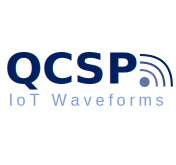
\includegraphics[width=\textwidth]{QCSP_Logo.pdf}
        \end{column}
        \begin{column}{.2\linewidth}
          \includegraphics[width=\linewidth]{anr_approved.jpg}
        \end{column}
      \end{columns}
      \small \vspace{5pt} Projet ANR \texttt{ANR-19-CE25-0013-01}
    \end{column}
    \begin{column}{.5\linewidth}
      \emph{``L'objectif du projet QCSP est de contribuer à l'évolution des réseaux IoT en établissant,
        en mettant en œuvre et testant un nouveau type de modulation codée.''}
    \end{column}
  \end{columns}

  \vspace{2 em}

  \begin{center}
    Partenaires :\\
    \includegraphics[width=0.6\linewidth]{figures/logos-thesis/partners-logos.png}
  \end{center}
\end{frame}

\begin{frame}{\acrfull{ccsk}}
  {}
  % \begin{overlayarea}{\linewidth}{.02 \textheight}
  % \end{overlayarea}
  \begin{overlayarea}{\linewidth}{.15 \textheight} \centering
    symboles de $p$ bits $\Longrightarrow$ rotation circulaire d'une \emph{séquence de pseudo-bruit binaire} (\acrshort{pn}) \cite{dillardCyclicCodeShift2003}.\\
    La \acrshort{pn} (noté \pn{0}) est composée $2^p = q$ \emph{chips}, telle que $\mpn{0} = [P_0(0), ..., P_0(q - 1)]$
  \end{overlayarea}

  \begin{columns}
    \begin{column}{.3\linewidth}
      \begin{overlayarea}{\linewidth}{.37 \textheight}
        \centering

        \begin{tabular}{@{}r r l@{}}
          \toprule
          \multicolumn{3}{c}{\textbf{Paramètres}}         \\ \midrule
          $p$    & $=$ & $2$ bits par symbole             \\
          $q$    & $=$ & $4$ symboles possibles           \\
          \pn{0} & $=$ & \Ob{}\Xb{}\Xb{}\Xb{} ($4$ chips) \\
          \bottomrule
        \end{tabular} \vspace*{-2pt}

        \Ob{} $= 1$, \Xb{} $= 0$
      \end{overlayarea}
    \end{column}
    \begin{column}{.3\linewidth}
      \begin{overlayarea}{\linewidth}{.37 \textheight}
        \begin{tabular}{@{}r c l@{}}
          \toprule
          \textbf{Symbole} & \textbf{Notation} & \textbf{Rotation}    \\ \midrule
          $0$              & \pn{0}            & \Ob{}\Xb{}\Xb{}\Xb{} \\
          $1$              & \pn{1}            & \Xb{}\Ob{}\Xb{}\Xb{} \\
          $2$              & \pn{2}            & \Xb{}\Xb{}\Ob{}\Xb{} \\
          $3$              & \pn{3}            & \Xb{}\Xb{}\Xb{}\Ob{} \\
          \bottomrule
        \end{tabular}
      \end{overlayarea}
    \end{column}
  \end{columns}

  \vspace{1 em}

  \begin{columns}
    \begin{column}{.35\linewidth}
      \begin{overlayarea}{\linewidth}{.19 \textheight}
        \centering
        Mot de code $\vect{C}$ de $3$ symboles\\
        $\{ 0, \; 3, \; 1\}$
      \end{overlayarea}
    \end{column}
    \begin{column}{.05\linewidth}
      \centering
      $\Rightarrow$
    \end{column}
    \begin{column}{.6\linewidth}
      \begin{overlayarea}{\linewidth}{.19 \textheight}
        \centering
        % \begin{noindent}
        \begin{tabular}{@{}r c@{}}
          \multicolumn{2}{c}{Trame \acrshort{ccsk} $\vect{F}_{CCSK}$}          \\
          $\{ \mpn{0} \;|\; \mpn{3} \;|\; \mpn{1} \}$ = 
            & {\large \Ob{}\Xb{}\Xb{}\Xb{}~~\Xb{}\Xb{}\Xb{}\Ob{}~~\Xb{}\Ob{}\Xb{}\Xb{}} \\
            & \includegraphics[width=.387\linewidth, height=.05\textheight]{figures/tikzpicture/pn_chrono.pdf}
        \end{tabular}
        % \end{noindent}
      \end{overlayarea}
    \end{column}
  \end{columns}
  \begin{columns}
    \begin{column}{.6678\linewidth}
      Après le CCSK, on applique une BPSK ($1 \rightarrow +1$, $0 \rightarrow -1$) :
    \end{column}
    \begin{column}{.2322\linewidth} \centering
      \includegraphics[width=\linewidth, height=.1\textheight]{figures/tikzpicture/pn_chrono_bpsk.pdf}
    \end{column}
    \begin{column}{.055\linewidth}
    \end{column}
  \end{columns}
  \blfootnotetext{\textcite{dillardCyclicCodeShift2003}}
  % \footnotetext{Corps de Galois d'ordre $p$}
\end{frame}

\begin{frame}{\acrshort{ccsk} : Démodulation}
  {\scriptsize Note : Post BPSK, donc cette fois, \Ob{} $= +1$, \Xb{} $= -1$.}

  Corrélation circulaire $\vect{L}$: $\quad\forall k \in \llbracket 0, q - 1 \rrbracket, \quad L(k) = \sum_{i = 0}^{q - 1} y(i) \times P_0(k + i \mod{q})$. \vspace{-2pt}
  \begin{center}
    On note $\vect{y} = \mgb{} \mgb{} \mgb{} \mgb{}$, avec ``$\mgb{}$'' une valeur quelconque.
  \end{center} \vspace{-5pt}
  \begin{columns}
    \begin{column}{.25\linewidth}
      \centering
      \ra{.5}
      \begin{tabular}{@{}r l@{}}
        $L(0) =$ &
        \begin{tabular}{@{}c l@{}}
          $\mgb{} \pta{} \mgb{} \pta{} \mgb{} \pta{} \mgb{}$ \\
          $\times + \times + \times + \times$                \\
          $\mOb{} \pta{} \mXb{} \pta{} \mXb{} \pta{} \mXb{}$
        \end{tabular}
      \end{tabular}
      \ra{1}
    \end{column}
    \begin{column}{.25\linewidth}
      \centering
      \ra{.5}
      \begin{tabular}{@{}r l@{}}
        $L(1) =$ &
        \begin{tabular}{@{}c@{}}
          $\mgb{} \pta{} \mgb{} \pta{} \mgb{} \pta{} \mgb{}$ \\
          $\times + \times + \times + \times$                \\
          $\mXb{} \pta{} \mOb{} \pta{} \mXb{} \pta{} \mXb{}$
        \end{tabular}
      \end{tabular}
      \ra{1}
    \end{column}
    \begin{column}{.25\linewidth}
      \centering
      \ra{.5}
      \begin{tabular}{@{}r l@{}}
        $L(2) =$ &
        \begin{tabular}{@{}c@{}}
          $\mgb{} \pta{} \mgb{} \pta{} \mgb{} \pta{} \mgb{}$ \\
          $\times + \times + \times + \times$                \\
          $\mXb{} \pta{} \mXb{} \pta{} \mOb{} \pta{} \mXb{}$
        \end{tabular}
      \end{tabular}
      \ra{1}
    \end{column}
    \begin{column}{.25\linewidth} \centering
      \ra{.5}
      \begin{tabular}{@{}r l@{}}
        $\vect{L} =$ &
        \begin{tabular}{@{}c@{}}
          $\mgb{} \pta{} \mgb{} \pta{} \mgb{} \pta{} \mgb{}$ \\
          $\times + \times + \times + \times$                \\
          $\mXb{} \pta{} \mXb{} \pta{} \mXb{} \pta{} \mOb{}$
        \end{tabular}
      \end{tabular}
      \ra{1}
    \end{column}
  \end{columns}

  \vspace{15pt}

  \begin{columns}
    \begin{column}{.25\linewidth}
      \captionof{figure}{$\vect{y} = \mpn{0}$ \\ Autocorrélation circulaire de \pn{\textcolor{Red}{\bm{0}}}}
      \includegraphics[width=\linewidth]{pgfplots/pn_demod_0.pdf}
    \end{column}
    \begin{column}{.25\linewidth}
      \captionof{figure}{$\vect{y} = \mpn{1}$ \\ Corrélation circulaire de \pn{0} et \pn{\textcolor{Red}{\bm{1}}}}
      \includegraphics[width=\linewidth]{pgfplots/pn_demod_1.pdf}
    \end{column}
    \begin{column}{.25\linewidth}
      \captionof{figure}{$\vect{y} = \mpn{2}$ \\ Corrélation circulaire de \pn{0} et \pn{\textcolor{Red}{\bm{2}}}}
      \includegraphics[width=\linewidth]{pgfplots/pn_demod_2.pdf}
    \end{column}
    \begin{column}{.25\linewidth}
      \captionof{figure}{$\vect{y} = \mpn{3}$ \\ Corrélation circulaire de \pn{0} et \pn{\textcolor{Red}{\bm{3}}}}
      \includegraphics[width=\linewidth]{pgfplots/pn_demod_3.pdf}
    \end{column}
  \end{columns}
\end{frame}

\end{document}
